\chapter[SCP-077 腐颅]{
    SCP-077 Rot Skull\\
    SCP-077 腐颅
}

\label{chap:SCP-077}

\begin{figure}[H]
    \centering
    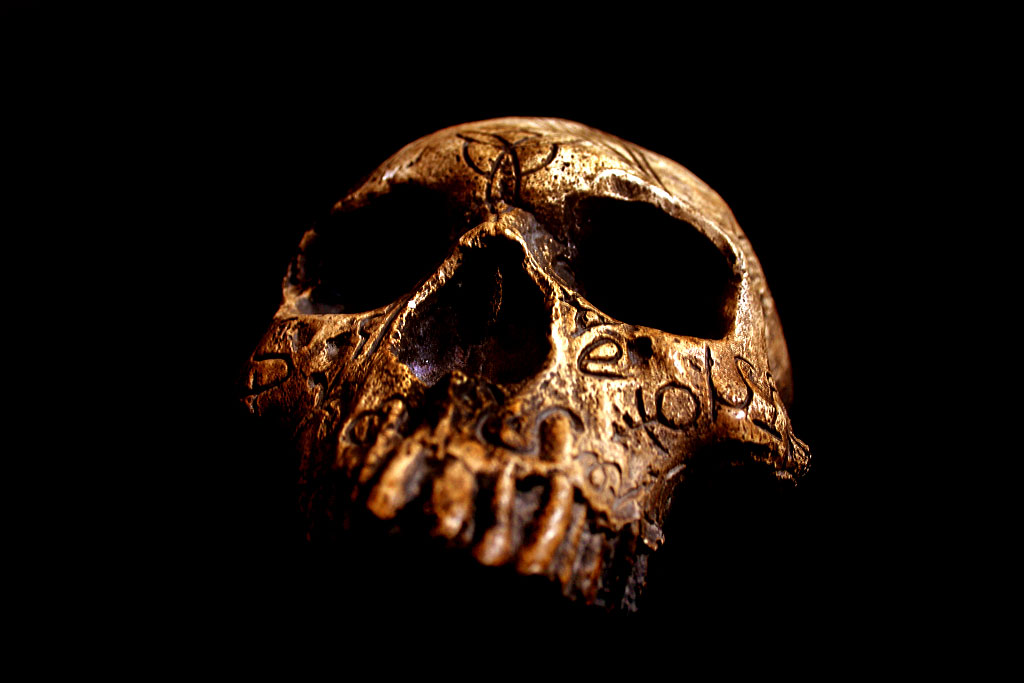
\includegraphics[width=0.5\linewidth]{images/SCP.077.jpg}
    \caption*{在被诵读前的SCP-077。}
\end{figure}

\bb{项目编号:}SCP-077

\bb{项目等级:}Euclid

\bb{特殊收容措施:}SCP-077被收容于Sector-86内一的0.5m钢制底座上,至于一3m x 3m x 3m的收容间内,配有0.5m厚的钢制强化墙壁。强化钢舱门遵照AH37-协议,由两(2)名1级人员全天守卫。一台摄像头将监控房间内部确认是否出现异变。

每八(8)小时一次,一对至少两(2)人(推荐三(3)人)的受训D级人员将进入收容区并大声、清楚地朗读上雕刻的符文。阅读须由理解所读符文完整含义的D级人员进行,读时要保持发音正确,且距离SCP-077有30cm远。

所有人员必须接受一星期的训练课程,由基金会语言学家指导其发音、阅读和方言辅导。最少二十(20)名D级人员要保持接受全天训练;受训D级人员将免除处决直至被替换。基金会语言学家须待命以备出现出乎预测的符文变化。每一次符文更新都需尽快地被抄录为书面英文,包括文字版和方便理解的翻译版;参见文件077-██████到██████查阅过往翻译。

Research Sector-861的自助餐厅不得提供土豆或含土豆的菜品。

\bb{描述:}SCP-077是一人类头骨的上半部分,其上刻有符文,符文刻槽内填有一种未辨识的黑色树脂。这些符文会在每个月亮月(定义为满月升起于爱尔兰地平线的时间)、冬夏至、春秋分、以及可从爱尔兰观测到的任何程度日月食发生时发生变化。

若雕刻的文字未能在24小时内被大声读出, SCP-077的眼窝和鼻腔内会开始释放SCP-077-1。SCP-077-1是一种发光绿色气体,尚不清楚其确切性质;值得注意的是SCP-077-1一般表现地与普通气体无差别,但它只会停留于SCP-077的有效“视野”内,除非空间受限不会流动到SCP-077的后方。不透明、不通透且无生物成分的障碍可以暂时阻挡SCP-077-1;然而试图将SCP-077永久收容于不透明容器内未能成功,因其产生的SCP-077-1过多,足以撑破容器。

生物材料(SCP-077自身当然除外)若接触到SCP-077-1,将被立即转化为一种粘性的恶臭粘浆;粘浆被确认为腐烂的土豆块茎(\ii{Solanum tuberosum}),且均已感染严重土豆晚疫病(\ii{Phytophthora infestans})。一(1)立方米的SCP-077-1至多可转化掉八百(800)克的生物材料。

阅读SCP-077上的符文会对阅读者的健康造成显著影响。影响包括恶心、痉挛、头痛、头晕、失禁、发烧、皮疹、鼻出血、意识模糊等。这些影响会随阅读时间增加而变强,若连续和\slash 或频繁阅读多次还可能出现累积。阅读者有60\%的概率出现土豆过敏。

\bb{附录077-01:}\\
该物品发现于爱尔兰{[}删除]村的█████ █████████。当地人为该物品建立了一座神龛,最多有{[}删除]名参与者每夜进行仪式。

从村中教堂(参见归档077-1576)和图书馆(参见归档077-1582)内回收到历史文件残片,其中记载该物体最早可追溯到1848年,当时对该物品德描述中使用了很多褒义词汇-包括“守护者”、{[}删除]等。然而到了1869年,对该物品的提及都是委婉地表达恐惧和愤恨。
